\documentclass{beamer}

\usepackage{amsmath, amssymb}
\usepackage{graphicx}
\usepackage{url}
\usepackage{xspace}
\usepackage{pifont}
\usepackage{minted}
\usepackage{verbatim}
\usepackage{wasysym}
\usepackage[numberedbib]{apacite}
\usepackage{bm}

\DeclareMathOperator{\Tr}{Tr}

\usetheme{AnnArbor}
\usefonttheme[onlymath]{serif}

\title[Intro DNNs]{\textbf{Practical Deep Neural Networks} \\
\textbf{\normalsize GPU computing perspective}\\
\normalsize Recurrent Neural Networks}
\author{Yuhuang Hu \and Chu Kiong Loo}
\institute[UM]{Advanced Robotic Lab\\
Department of Artificial Intelligence\\
Faculty of Computer Science \& IT\\
University of Malaya}

\date{}

\begin{document}

\frame{\titlepage}

\begin{frame}
  \frametitle{Outline}

  \tableofcontents
\end{frame}

\AtBeginSection[]
  {
     \begin{frame}
     \frametitle{Outline}
     \tableofcontents[currentsection]
     \end{frame}
  }

\section{Introduction}

\begin{frame}
  \frametitle{Assumed prerequisites}

  \begin{itemize}
    \item[\ding{80}] Neural Computation (DL book chapter 4)
    \item[\ding{80}] Machine Learning Basics (DL book chapter 5)
    \item[\ding{80}] MLP Networks (DL book chapter 6)
  \end{itemize}
\end{frame}

\begin{frame}
  \frametitle{Suggest Readings}

  \begin{itemize}
    \item[\ding{45}] Deep Learning book \href{http://www.iro.umontreal.ca/~bengioy/dlbook/rnn.html}{Chapter 10: Sequence Modeling: Recurrent Recursive Nets}
    \item[\ding{45}] CS224d: \href{http://cs224d.stanford.edu/lectures/CS224d-Lecture8.pdf}{GRUs and LSTMs -- for machine translation}
    \item[\ding{45}] \href{http://karpathy.github.io/2015/05/21/rnn-effectiveness/}{The Unreasonable Effectiveness of Recurrent Neural Networks}
    \item[\ding{45}] \href{http://arxiv.org/abs/1503.04069}{LSTM: A Search Space Odyssey}
    \item[\ding{45}] \href{http://www.cs.toronto.edu/~graves/preprint.pdf}{Supervised Sequence Labelling with Recurrent Neural Networks}
  \end{itemize}
\end{frame}

\section{SRN}

\begin{frame}
  \frametitle{SRN architecture}
  
  \begin{figure}
    \centering
    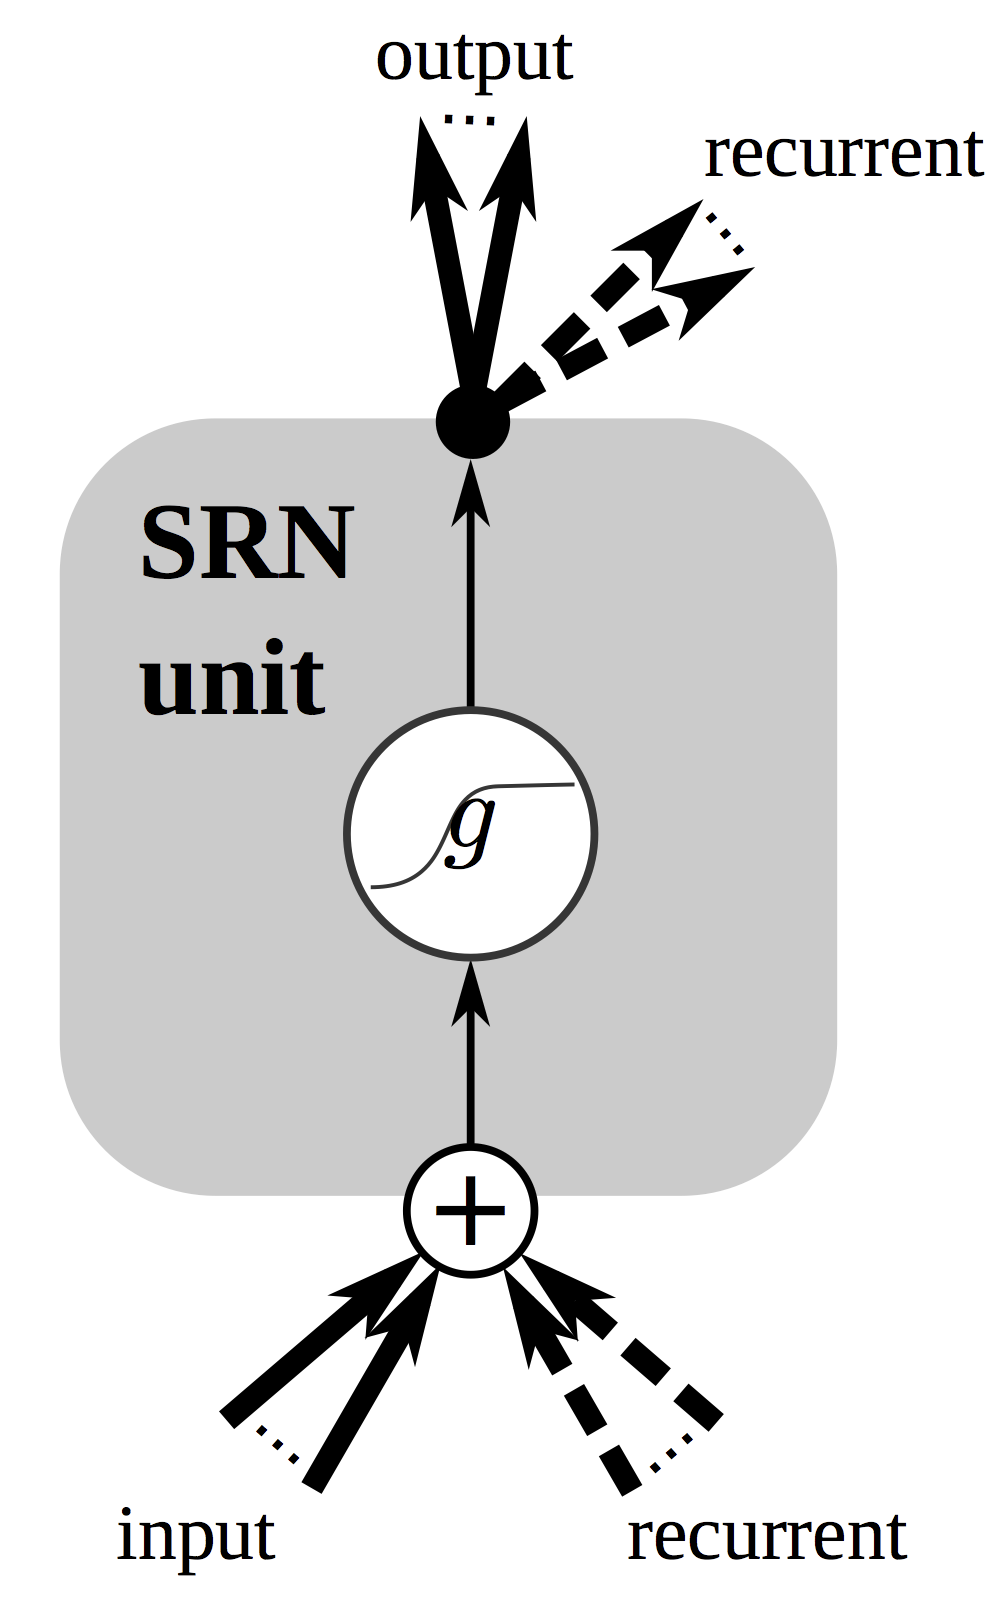
\includegraphics[width=0.3\textwidth]{srn_architecture.png}
  \end{figure}
\end{frame}

\begin{frame}
  \frametitle{SRN architecture}

  \begin{align*}
    \mathbf{y}_{h}^{t}&=f_{h}(\mathbf{W}_{i}\mathbf{x}^{t}+\mathbf{W}_{h}\mathbf{y}^{t-1}) \\
    \mathbf{y}_{o}^{t}&=f_{o}(\mathbf{W}_{o}\mathbf{y}_{h}^{t})
  \end{align*}
  where $\mathbf{W}_{h}$, $\mathbf{W}_{i}$, $\mathbf{o}$ are the hidden, input and output weight matrices, $\mathbf{x}^{t}$ is the input vector, and $\mathbf{y}_{h}^{t}$ is a vector representing the activation of hidden units at time step $t$. Functions $f_{h}(\cdot)$ and $f_{o}(\cdot)$ are non-linear functions.
\end{frame}

\section{LSTM}

\begin{frame}
  \frametitle{LSTM architecture}
  
  \begin{figure}
    \centering
    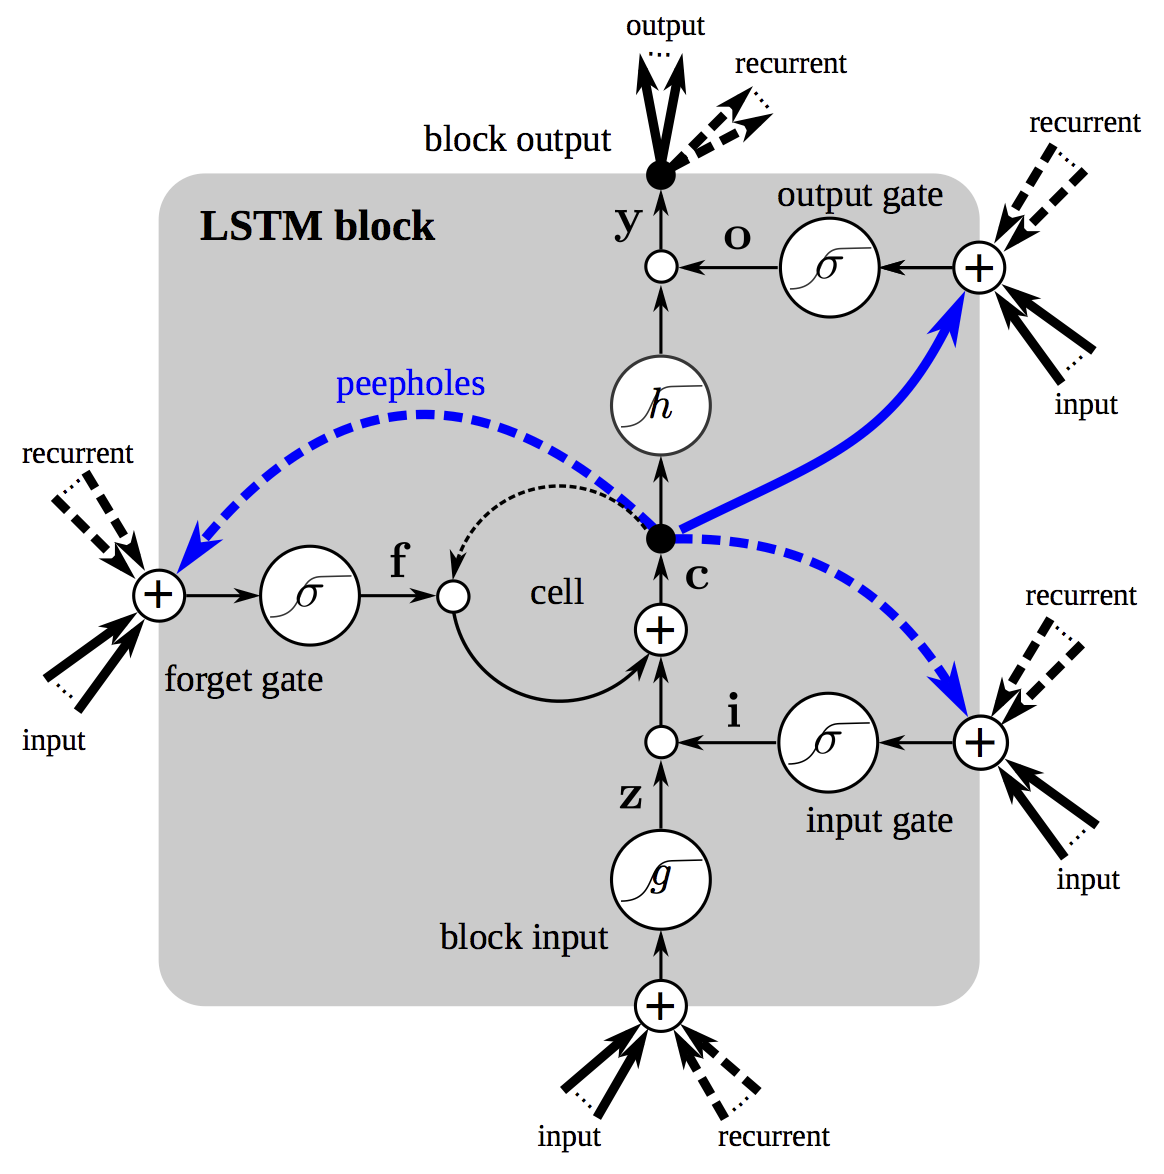
\includegraphics[width=0.6\textwidth]{lstm_architecture.png}
  \end{figure}
\end{frame}

\begin{frame}
  \frametitle{LSTM architecture}

  \begin{equation*}
    \begin{array}{lr}
      \mathbf{z}^{t}=g(\mathbf{W}_{z}\mathbf{x}^{t}+\mathbf{R}_{z}\mathbf{y}^{t-1}+\mathbf{b}_{z}) & \text{\emph{block input}} \\
      \mathbf{i}^{t}=\sigma(\mathbf{W}_{i}\mathbf{x}^{t}+\mathbf{R}_{i}\mathbf{y}^{t-1}+\mathbf{p}_{i}\odot\mathbf{c}^{t-1}+\mathbf{b}_{i}) & \text{\emph{input gate}} \\
      \mathbf{f}^{t}=\sigma(\mathbf{W}_{f}\mathbf{x}^{t}+\mathbf{R}_{f}\mathbf{y}^{t-1}+\mathbf{p}_{f}\odot\mathbf{c}^{t-1}+\mathbf{b_{f}}) & \text{\emph{forget gate}} \\
      \mathbf{c}^{t}=\mathbf{i}^{t}\odot\mathbf{z}^{t}+\mathbf{f}\odot\mathbf{c}^{t-1} & \text{\emph{cell state}} \\
      \mathbf{o}^{t}=\sigma(\mathbf{W}_{o}\mathbf{x}^{t}+\mathbf{R}_{o}\mathbf{y}^{t-1}+\mathbf{p}_{o}\odot\mathbf{c}^{t}+\mathbf{b}_{o}) & \text{\emph{output gate}} \\
      \mathbf{y}^{t}=\mathbf{o}^{t}\cdot h(\mathbf{c}^{t}) & \text{\emph{block output}}
    \end{array}
  \end{equation*}
  Here $\mathbf{x}^{t}$ is the input vector at time $t$, the $\mathbf{W}$ are rectangular matrices, the $\mathbf{R}$ are square recurrent weight matrices, the $\mathbf{p}$ are peehole weights vectors and $\mathbf{b}$ are bias vectors. Functions $\sigma$, $g$ and $h$ are point-wise non-linear activation functions: \emph{logistic sigmoid} is used for as activation function of the gates and \emph{hyperbolic tangent} is usually used as the block input and output activation function. The point-wise multiplication of two vectors is denoted with $\odot$
\end{frame}

\section{Sequence Modeling}

\begin{frame}
  \frametitle{Modes of Processing}

  \begin{figure}
    \centering
    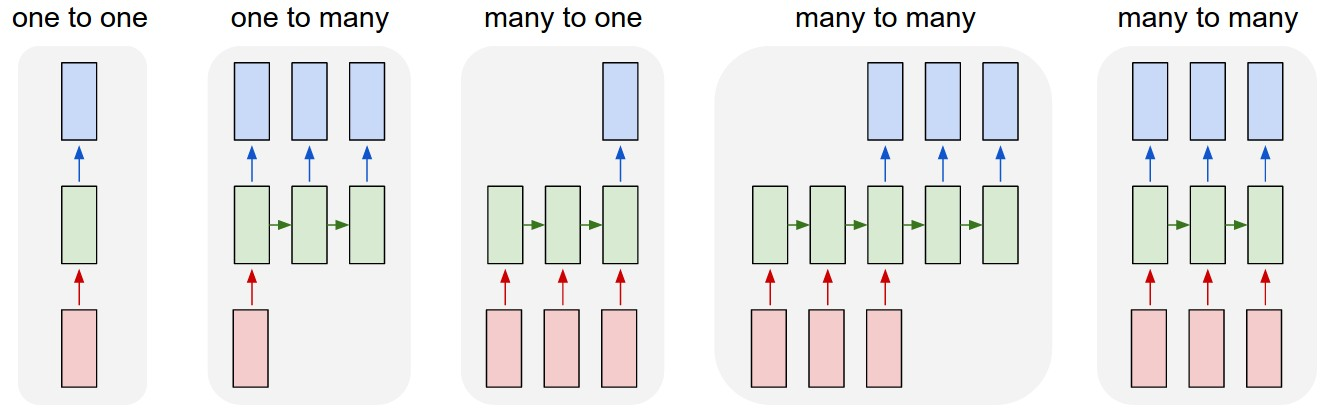
\includegraphics[width=0.9\textwidth]{diags.jpeg}
  \end{figure}

  Left to right: \textbf{(a)} fixed-size input to fixed-size output (\emph{e.g.} image classification); \textbf{(b)} sequence output (\emph{e.g.} image captioning); \textbf{(c)} sequence input (\emph{e.g.} sentiment analysis); \textbf{(d)} sequence input and sequence output (\emph{e.g.} machine translation); \textbf{(e)} synced sequence input and output (\emph{e.g.} video classification)
\end{frame}

\begin{frame}
  \frametitle{Example: character prediction}

  \begin{figure}
    \centering
    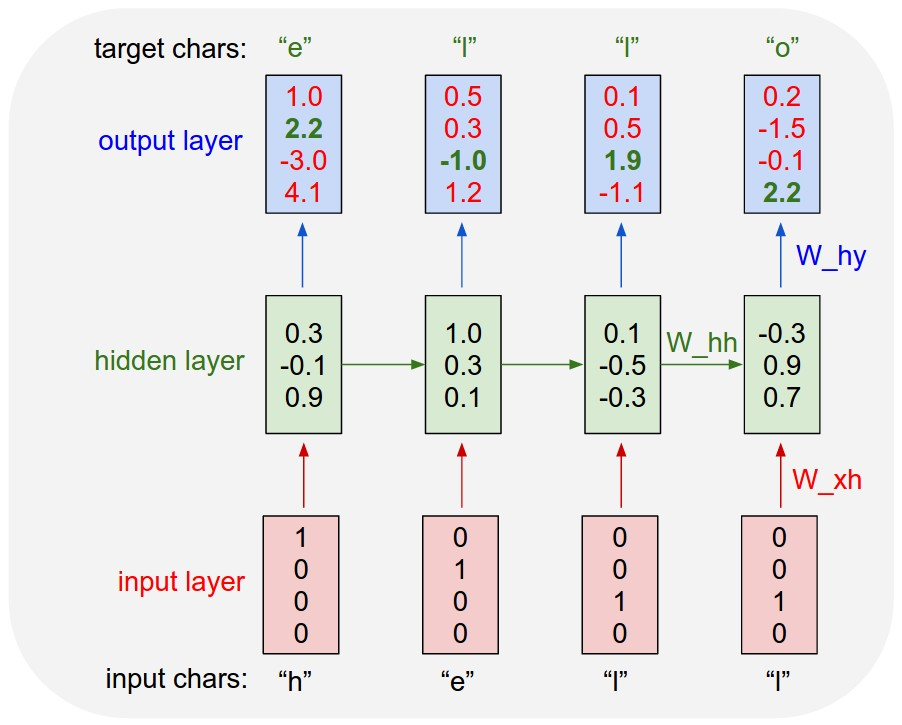
\includegraphics[width=0.65\textwidth]{charseq.jpeg}
    \caption{Predict ``hello''}
  \end{figure}
\end{frame}

\begin{frame}
  \frametitle{Example: image captioning}

  \begin{figure}
    \centering
    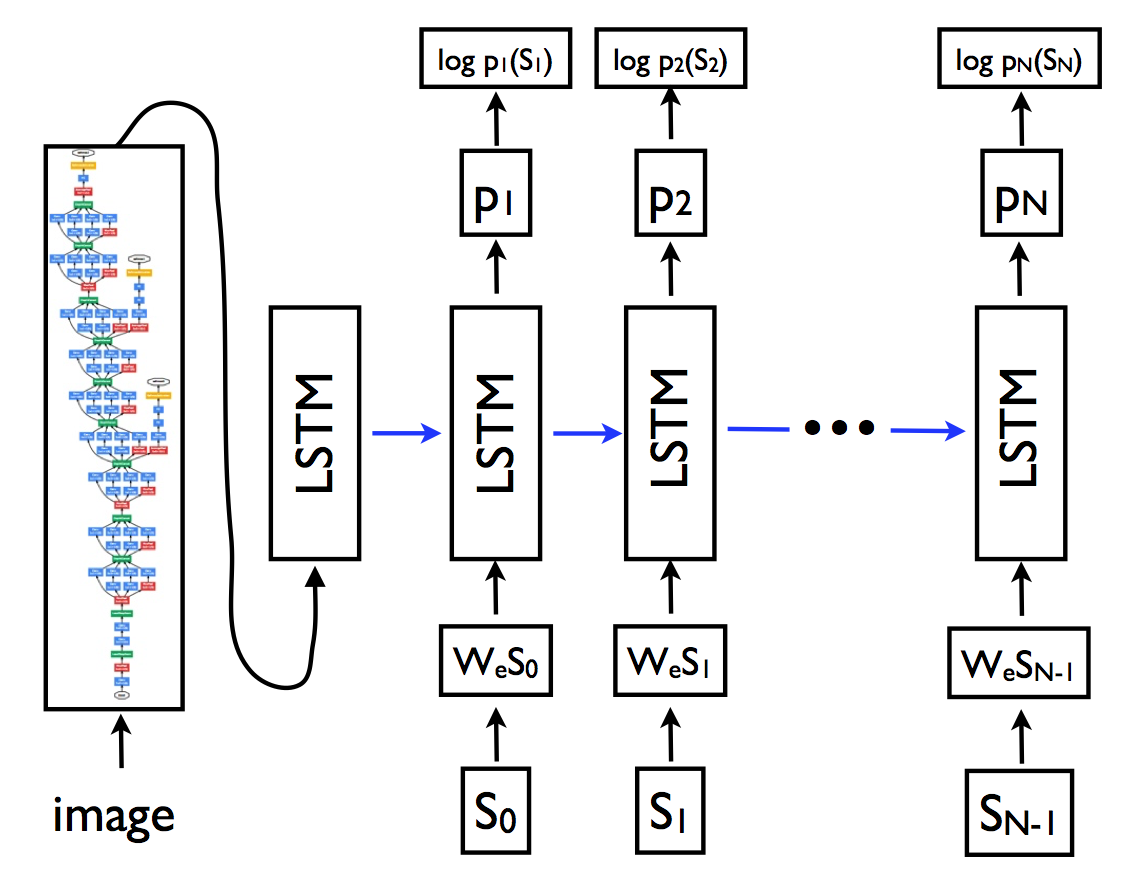
\includegraphics[width=0.6\textwidth]{image_captioning.png}
  \end{figure}
\end{frame}

\section{Q\&A}

\begin{frame}
  \frametitle{Q\&A}

  \begin{figure}[!htm]
    \centering
    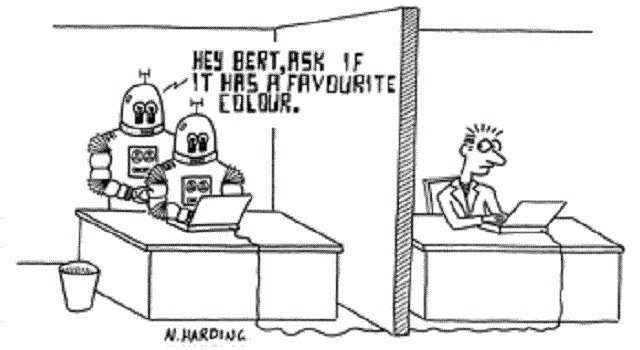
\includegraphics[width=0.7\textwidth]{turingtest.jpg}
  \end{figure}
\end{frame}

\end{document}
%%% Local Variables:
%%% mode: latex
%%% TeX-master: t
%%% End:
